\documentclass[../main.tex]{subfiles}
\begin{document}

\chapter{Lecture 20 - 19-05-2020}

\section{Support Vector Machine Analysis}

$$
\min_{w \in \barra{R}} \frac{1}{2}
 \| w\|^2 \qquad s.t \quad y_t \, w^T \, x_t \geq 1 \ t =1 ,...,m$$
 $$
 \max_{\gamma >0} \gamma^2 \qquad s.t. \quad \|u\|^2 < 1 (?) \quad y_t \, u^T \, x_t \geq \gamma \ t = 1,...,m
 $$
 The two are kinda equivalent
 $$
 y_t \left( \frac{u}{\gamma}^2  \right) x_t \geq 1 \ t=1,...,m \qquad w = \frac{u}{\gamma} \qquad \|u\|^2 = \|w\|^2 \gamma^2 = 1, \ \gamma^2 = \frac{1}{\|w\|^2}
 $$
 $$
 \max \frac{1}{\|w\|^2} \rightsquigarrow \min \|w\|^2 \qquad w^* = \frac{u^*}{\gamma^*}
 $$
 $$
 \gamma^2 \| w\|^2 = 1 \textit{ is redundant!} \qquad y_t w^T x_t \geq 1 \ t=1,...,m
 $$
What we do with $w^*$?
\\
\subsection{Fritz John Optimality Conditions}
$$
\min_{w \in \barra{R}^d} f(w) \quad s.t \quad g_t(w) \leq 0 \ t=1,...,m \qquad \textit{ $f,g_1,..,g_m$ all differentiable}
$$
If $w_0$ is optimal solution, then $\exists \alpha = (\alpha_1,...,\alpha_m) \in \barra{R}^m$
\\
$$
\nabla f(w_0) + \sum_{t  \in I} \alpha_t \nabla g_t (w_0) = 0 \qquad I = \{ t : g_t(w_0) = 0 \}
$$
$$
f(n) = \frac{1}{2} \| w \|^2 \qquad g_t(w)=  1 - y_t \, w^T \, x_t, \ \nabla g_t(w^*) =  - y_t \, x_t
$$
$w^*$ SVM solution
$$
w^* - \sum_{t \in I} \alpha_t y_t x_t = 0 \ \ \Leftrightarrow \ \ w^* = \sum_{t \in I} \alpha_t y_t x_t
$$
where $f(n) = \nabla f(w^*)$
$$
I = \{ \, t : y_t(w^*)^T \, x_t = 1 \} \textbf{ support vectors}
$$
We want a generalisation of this two non separable training set.
\\
\subsection{Non-separable case}
$$
\min_{w \in \barra{R}^d} \frac{1}{2}
 \| w\|^2 \qquad s.t \quad y_t\, w^T \, x_t \ \geq 1$$
We cannot satisfy all the constraints since are inconsistent. Maybe we can try to satisfy the most possible constrain so:
$$
\min_{w \in \barra{R}^d} \frac{1}{2}
 \| w\|^2  + \frac{1}{2} \sum_{t=1}^m \xi_t \qquad
 y_t\, w^T \, x_t \ \geq 1- \xi_t
$$
where $\xi_t$ slack variables and $ \xi > 0$
We want $\xi_t$ given $w$:
$$
\xi_t =  \begin{cases}
1- y_t \, w^T \, x_t \qquad if \ y_t \, w^T x_t < 1
\\
0 \qquad otherwise
\end{cases} \qquad \xi_t = \left[ 1- y_t \, w^T \, x_t \right] = h_t(w) \ \textit{ hinge loss}
$$
We replate this in the first equation and we get a convex function plus $\lambda$-SC function:
$$
\min_{w \in \barra{R}^d} F(w) \qquad F(w) = \frac{1}{m} \sum_{t = 1}^m h_t(w) + \frac{1}{2}
\| w\|^2 $$
And this is unconstrained and $F(W)$ is $\lambda$-S.C.
\\\\
I also want to check my shape of the function is not changing. 
\\ 
Assume I can write the solution as:
$$
w^* = \sum_{t=1}^m \alpha_t \, y_t \, x_t + u 
$$
where $u$ is orthogonal to each of $x_1,...,x_m$
$
 \sum_{t=1}^m \alpha_t \, y_t \, x_t \ = \ v
 $
$$
 w^* = v + u \qquad v = w^* - u \quad \|v \| \leq \| w^*\|
$$
\begin{figure}[h]
    \centering
    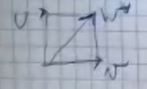
\includegraphics[width=0.3\linewidth]{../img/lez20-img1.JPG}
    \caption{}
    %\label{fig:}
\end{figure}\\
\\
Now I can check the hinge loss:
$$
h_t(v) = \left[ 1- y_t(w^*)^* x_t+  \red{y_t \, u^T \, x_t} \right]_+ = h_t(w^*)
$$
Since $y_t \, u^T \, x_t = 0$ this cancel out and we get the hinge loss.
$$
F(v) = \frac{1}{m} \sum_t h_t(w^*) + \frac{1}{2} \| w\|^2 \leq F(w^*)
$$
$$
w^* = \sum_{t=1}^m \alpha_t y_t x_t \qquad \alpha_t \neq 0 \ \Leftrightarrow \ h_t(w^*) > 0
$$
Including $t : y_t(w^*)^T x_t = 1$\\
\begin{figure}[h]
    \centering
    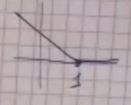
\includegraphics[width=0.2\linewidth]{../img/lez20-img2.JPG}
    \caption{}
    %\label{fig:}
\end{figure}\\
\\
Support vector are those in which I need slack variables in order to be satisfied.
\begin{figure}[h]
    \centering
    
\includegraphics[width=0.5\linewidth]{../img/lez20-img3.JPG}
    \caption{}
    %\label{fig:}
\end{figure}\\
\\
$$
F(w) = \frac{1}{m} \sum_{t=1}^m h_t(w) + \frac{1}{2} \| w\|^2  = \frac{1}{m} \sum_{t=1}^m \ell_t(w)
$$
MANCA FORMULAA\\
We need to minimise the hinge loss and we use Pegasos.
\section{Pegasos: OGD to solve SVM}
Stochastic gradiant descent.
\\\\
Parameters: $ \lambda > 0$, $T$ number of rounds
\\
Set $w_1 =(0,...,0)$
\\
For $t = 1,...,T$
\\
1) Draw $(x_{zt}, y_{zt})$ at random from training set
\\
2) $w_{t+1} = w_t - \eta_t \nabla \ell_{zt}(w_t)$
\\
Output $\bar{w} = \frac{1}{T} \sum_t w_t$
$$
\ell_{zt}(w) = h_{zt} (w) + \frac{1}{2} \| w\|^2 \qquad w^* = arg \min_{w \in \barra{R}^*} \left( \frac{1}{m} \sum_{t=1}^m h_t(w) + \frac{\lambda}{2} \| w\|^2\right)
$$
$\forall s_1,...,s_T$ realisation of $z_1,...,z_T$
$$
\frac{1}{T} \sum_{t=1}^m \ell_{st}(w_t) \leq \frac{1}{T}\sum_{t=1}^m \ell_{st} (w^*) + \frac{G^2}{2 \, \lambda \, T} \ln (T+1) \quad OGD\ Analysis
$$
$$
G = \max_t \| \nabla \ell_{st}(w_t) \|
$$
In general $G$ is random.
$$
F(\bar{w}) \leq F(w^*) + \varepsilon \qquad \| \bar{w}- w^*\| \ \leq^? \ | F(\bar{w}) - F(w^*) |  \ \leq \ L \| \bar{w} - w^* \|
$$
where $F$ is the average of the losses: $F(w_t) = \frac{1}{m} \sum_{s=1}^m \ell_s(w_t)$ \\
So we use Liptstik solution.
$$
\barra{E} \, [\ell_{zt}(w_t) | z_1,...,z_{t-1}] = \frac{1}{m} \sum_{s=1}^m \ell_s(w_t) \qquad \barra{E} \left[ \, X \, \right] = \barra{E} \left[ \, \barra{E} \left[ \, X | Y \, \right] \, \right]
$$
Now we use Jensen inequality:
$$
\barra{E} \, [ F(\bar{w} ) ] \ \leq^{J} \barra{E} \, \left[ \frac{1}{T} \sum_{t=1}^T F(w_t) \right] \ = \ \barra{E} \, \left[ \frac{1}{T} \sum_{t=1}^T \barra{E} \, \left[ \, \ell_{zt}(w_t) \, | \, z_1,...,z_{t-1} \, \right] \, \right]
\ = $$
$$
\ = \ \barra{E} \left[ \frac{1}{T} \sum^T_{t=1} \ell_{zt} (w_t) \right] \ \leq \ \barra{E} \left[ \frac{1}{T} \sum_{t=1}^T \ell_{zt}(w^*) \right] + \frac{\barra{E}[G^2]}{2 \, \lambda \, T} \ln (T+1) = 
$$ 
$$
=  \barra{E} \left[ \frac{1}{T} \sum_{t=1}^T \barra{E} [\ell_{zt}(w^*) | z_1,...,z_{t-1} ]\right] + \frac{\barra{E} [G^2]}{2 \, \lambda \, T} \ \ln \, (T+1) = 
$$
$$
= \barra{E} \left[ \frac{1}{T} \sum_{t=1}^T F(w^*) \right] + \frac{E[G^2]}{2 \, \lambda \, T} \ln (T+1) = \ = F(w^*) + \frac{\barra{E} [G^2]}{2 \, \lambda \, T} \ln (T+1)
$$
$\barra{E} [G^2] \leq ?
$
We are bounding $G^2 \ \forall s_1,..,s_T$
$$
\nabla \ell_{st}(w_t) = - y_{st} \, x_{st} \, I\{ h_{st}(w_t) >0\} + \lambda \, w\qquad \ell_s(w) = h_t(w) + \frac{1}{2} \|w\|^2
$$
$$
v_t = y_{st} \, x_{st} \, I \{ h_{st} (w_t) >0 \}, \quad \nabla \ell_{st}(w_t) = - v_t + \lambda w_t \quad \eta_t = \frac{1}{\lambda \, t}
$$
$$
w_{t+1} = w_t - \eta_t \nabla \ell_t(w_t) = w_t+ \eta_t \, v_t -\eta_t \, \lambda \, w_t = \left(1- \frac{1}{t} \right) w_t + \frac{1}{\lambda \, t} v_t=
$$ 
$$
\|\nabla \ell_{st}(w_t) \| \leq \| v_t \| + \lambda \| w_t \| \leq X + \lambda \|w_t\| \qquad X = \max_t \| x_t\|
$$
$$
w_{t+1} = \left( 1- \frac{1}{t} \right) w_t + \frac{1}{\lambda \, t} v_t \qquad w_1 = (0,...0) \quad w_t = \sum_t \beta_t v_t
$$
Fix $s <t$ \quad $\frac{1}{\lambda \, s} \sqrt[]{s} $
$$
\beta_s = \frac{1}{\lambda \, s} \prod^t_{r = s+1} \left( 1- \frac{1}{r} \right) = \frac{1}{\lambda \, s} \prod_{t = s+1}^t \frac{r-1}{r} = \frac{1}{\lambda \,  s} \frac{s}{t}
$$
$$
\frac{s}{s+1} \frac{s+1}{s+2}... \frac{t-1}{t} \qquad w_{t+1} = \frac{1}{\lambda \, t} \sum_{s=1}^t \sqrt[]{s}
$$
I know now that:
$$
\| \nabla \ell_{st}(w_t) \| \leq X + \lambda \|w_t \| \leq X_t \| \frac{1}{t} \sum_{s=1}^t \sqrt[]{s}\| \leq X + \frac{1}{t} \sum_{s=1}^t \| v_s \|
$$
$$
\| \nabla \ell_{st} (w_t) \| \leq 2 \, X \quad G^2 \leq 4\, x^2
$$
$$
\barra{E} [ F(\bar{w}] \leq F(w^*) + \frac{2 \, x^2}{\lambda \, T} \ln (T+1)
$$\\
General picture: Stochastic OGD, I can write my objective is an average of strongly  convex function. I sample for w
$$
F(w) = \frac{1}{m} \sum_{t=1}^m \ell_t(w)
$$
Then i get the expectation to links OGD to minisation of the objective.
\end{document}